Este capítulo descreve os procedimentos e as configurações feitas para a implementação empírica da metodologia deste trabalho.
Cada seção exibe um conjunto de gráficos relativos ao procedimento implementado para um único exemplo, os gráficos obtidos para todos
os exemplos se encontram no apêndice \ref{ApendiceA}.

\section{Configuração dos parâmetros}

As RIRSMs e AVCDs geradas nestes resultados usam as bases de dados de RIR, amostras de voz anecoicas e ruídos descritas no capítulo \ref{cap5}.
As faixas de DRR, T60 e SNR usados são exibidos na tabela \ref{tbl:config-param}.

\begin{table} [H]
    \centering
    \caption{Faixas dos parâmetros.}
    \label{tbl:config-param}
    \begin{tabular}{c|p{9cm}}

        \multicolumn{1}{c|}{\textbf{Parâmetro}} & \multicolumn{1}{c}{\textbf{Faixa}} \\
        \hline 

        $DRR_{alvo}$ (db) & $-6 \le DRR_{alvo} \le 18 $ \\
        $T60_{alvo}$ (s) & $T60_{org} - 1  \le T60_{alvo} \le T60_{org} + 1$ , onde o limite inferior de $T60_{alvo} = 0.2$ \\
        $SNR_{alvo}$ & $3 \le SNR_{alvo} \le 20 $ \\

    \end{tabular}
\end{table}

O $DRR_{alvo}$ segue os valores propostos no artigo \cite{RIR_Data_Aug}, já os valores de $T60_{alvo}$, devido à maior faixa de valores 
de $T60$ das RIRs base de AIR, são limitados a $\pm 1 $ segundo comparado ao valor de $T60_{org}$ da RIR usada durante a passagem do algoritmo.

\section{Resultados}

\subsection{\textit{Data Augmentation} do DRR}

Esta seção observa a eficácia da \textit{Data Augmentation} do DRR; para isso, foram gerados três exemplos de RIRSMs, suas configurações
são exibidas na tabela \ref{tbl:da-drr}, onde $DRR_{org}$ representa o DRR da RIR original, $DRR_{alvo}$ o valor de DRR desejado pelo usuário,
$DRR_{res}$ o valor de DRR obtido após DA e $\rho$ é o erro definido da forma $\rho = abs(DRR_{res} - DRR_{alvo})/DRR_{alvo}$.

\begin{table} [H]
    \centering
    \caption{Exemplos de DA de DRR gerados.}
    \label{tbl:da-drr}
    \begin{tabular}{c|c|c|c}

        \textbf{Exemplo} & 
        \textbf{Sala RIR} & 
        \textbf{Distância (m)} &
        \textbf{Amostra de Voz} \\
        \hline 

        D1 & lecture & 7.1 & H2-T2 \\
        D2 & booth & 1 & H2-T1 \\
        D3 & office & 2 & M2-T2 \\

    \end{tabular}
    \bigbreak
    \bigbreak
    \begin{tabular}{c|c|c|c|c}

        \textbf{Exemplo} & 
        \textbf{$DRR_{org}$ (db)} & 
        \textbf{$DRR_{alvo}$ (db)} &
        \textbf{$DRR_{res}$ (db)} & 
        \textbf{$\rho$ (\%)} \\
        \hline 

        D1 & -4,5 & 10 & 10 & 0 \\
        D2 & 4,7 & -2 & -2 & 0 \\
        D3 & 0,5 & 18 & 18 & 0 \\

    \end{tabular}
\end{table}


Nos exemplos gerados, na faixa determinada para o $DRR_{alvo}$, não houve diferença entre o $DRR_{alvo}$ e o $DRR_{res}$.
É possível observar na figura \ref{fig:rir-aug-d1} que ocorreu um aumento na seção equivalente a $h_e(t)$ comparado à figura \ref{fig:rir-og-d1}
para o exemplo D1.

\begin{figure} [H]
    \centering
    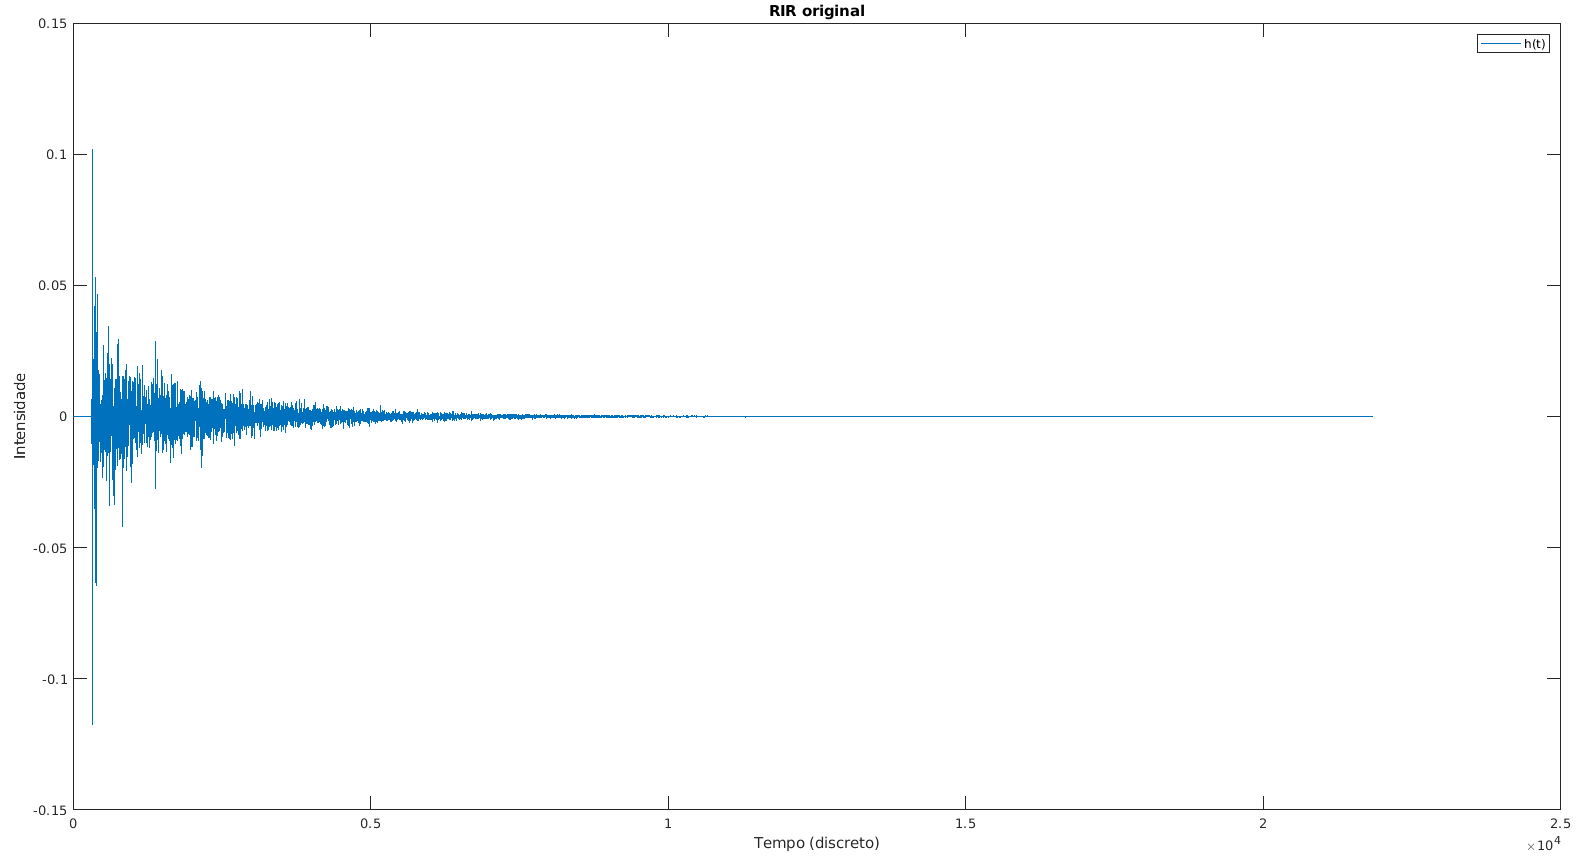
\includegraphics[scale=0.25]{rir-og-d1.png}
    \caption{RIR original do exemplo D1.}
    \label{fig:rir-og-d1}
\end{figure} 

\begin{figure} [H]
    \centering
    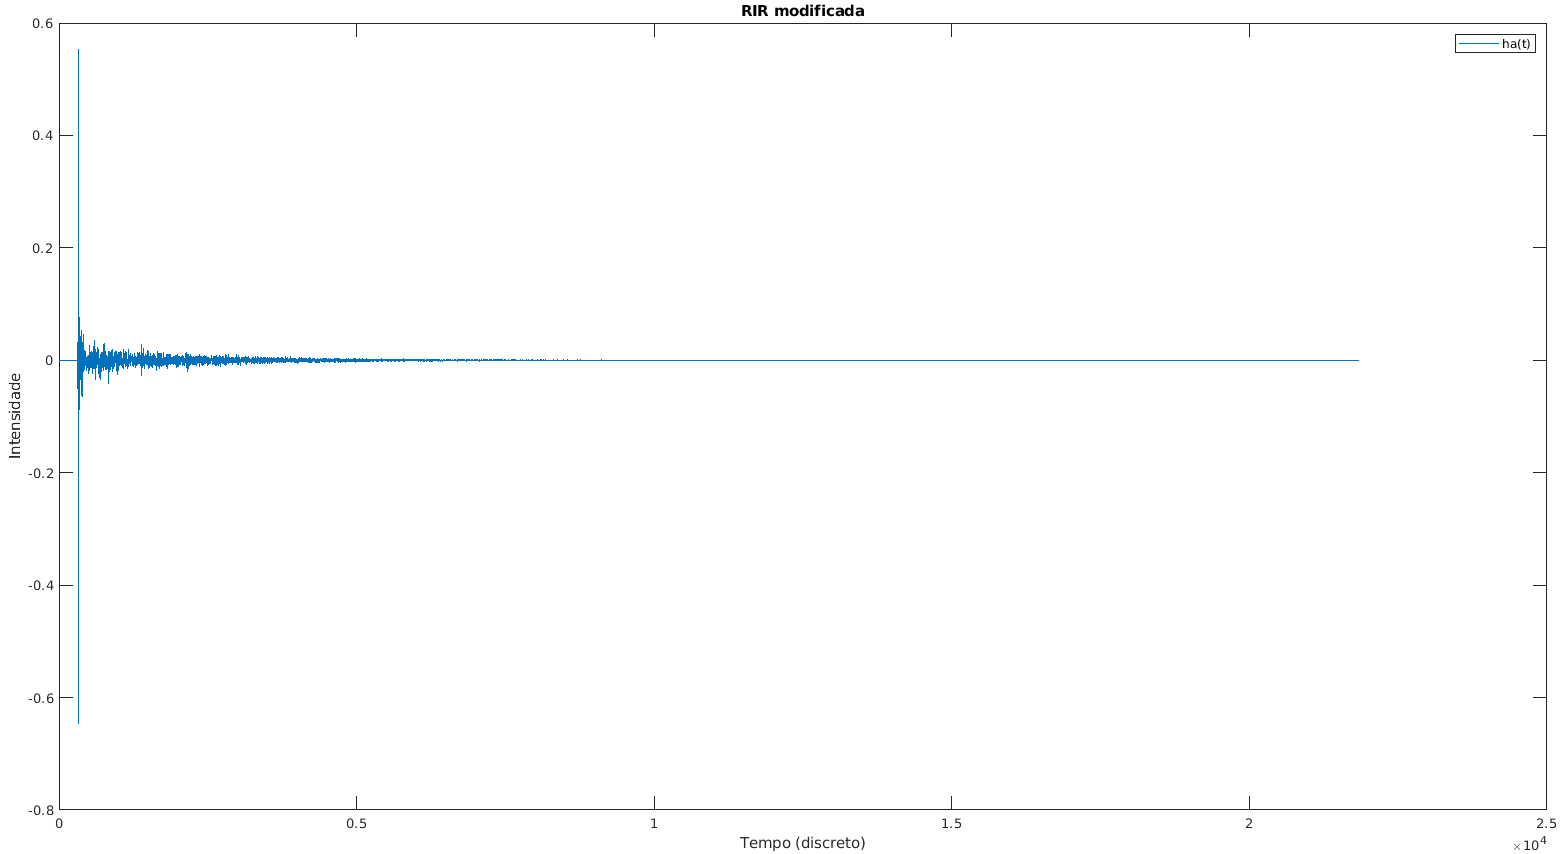
\includegraphics[scale=0.25]{rir-aug-d1.png}
    \caption{RIR simulada do exemplo D1.}
    \label{fig:rir-aug-d1}
\end{figure} 

Foi realizado também um experimento empírico com uma pessoa que não possui prévio conhecimento dos resultados gerados.
O objetivo desse experimento é medir o nível de “distância” do som, ou seja, a sensação subjetiva do locutor estar falando próximo ou distante
do microfone.
Foram geradas amostras de voz reverberadas (AVR) usando a RIROG e RIRSM e assim foram feitos dois testes subjetivos exibidos na tabela \ref{tbl:drr-exp}:
o primeiro, representado pela coluna “Comparação”, identifica qual das AVRs (a convoluída com RIROG ou a convoluída RIRSM) está mais distante;
já o segundo, representado pela coluna “Ordem”, identifica a ordem de mais para menos distante entre as AVRs geradas com RIRSMs.

\begin{table} [H]
    \centering
    \caption{Análise subjetiva de distância.}
    \label{tbl:drr-exp}
    \begin{tabular}{c|c|c|c|c}

        \textbf{Exemplo} & 
        \textbf{$DRR_{org}$ (db)} & 
        \textbf{$DRR_{res}$ (db)} & 
        \textbf{Comparação} &
        \textbf{Ordem} \\
        \hline 

        D1 & -4,5 & 10 & original & 2 \\
        D2 & 4,7 & -2 & simulado & 1 \\
        D3 & 0,5 & 18 & original & 3 \\

    \end{tabular}
\end{table}

De acordo com a tabela \ref{tbl:drr-exp}, foi possível identificar precisamente a diferença de variações do DRR para as RIRSMs.


\subsection{\textit{Data Augmentation} do T60}

Esta seção observa a eficácia da \textit{Data Augmentation} do T60; para isso, foram gerados três exemplos de RIRSMs, suas configurações
são exibidas na tabela \ref{tbl:da-t60}, onde $T60_{org}$ representa o T60 da RIR original, $T60_{alvo}$ o valor de T60 desejado pelo usuário,
$T60_{res}$ o valor de T60 obtido após DA e $\rho$ é o erro definido da forma $\rho = abs(T60_{res} - T60_{alvo})/T60_{alvo}$.

\begin{table} [H]
    \centering
    \caption{Exemplos de DA de T60 gerados.}
    \label{tbl:da-t60}
    \begin{tabular}{c|c|c|c}

        \textbf{Exemplo} & 
        \textbf{Sala RIR} & 
        \textbf{Distância (m)} &
        \textbf{Amostra de Voz} \\
        \hline 

        T1 & lecture & 7.1 & M2-T1 \\
        T2 & booth & 1 & H1-T2 \\
        T3 & office & 2 & H2-T2 \\

    \end{tabular}
    \bigbreak
    \bigbreak
    \begin{tabular}{c|c|c|c|c}

        \textbf{Exemplo} & 
        \textbf{$T60_{org}$ (s)} & 
        \textbf{$T60_{alvo}$ (s)} &
        \textbf{$T60_{res}$ (s)} & 
        \textbf{$\rho$ (\%)} \\
        \hline 

        T1 & 1,38 & 1,15 & 1,01 & 12.1 \\
        T2 & 1,01 & 1,88 & 1,89 & 0,5 \\
        T3 & 0,75 & 0,61 & 0,60 & 1,6 \\

    \end{tabular}
\end{table}

Nos exemplos gerados, na faixa determinada para o $T60_{alvo}$, foi observada uma mínima diferença entre o $T60_{alvo}$ e o $T60_{res}$ no exemplo T2 e T3;
já para o exemplo T1, notamos um erro considerável ao tentar reduzir o T60, o algoritmo proposto tem melhor acurácia para pequenas variações de T60 no caso de
redução, contudo o mesmo não é observado para o aumento do T60, mesmo com grandes variações entre $T60_{alvo}$ e $T60_{res}$.
É possível observar na figura \ref{fig:rir-aug-t2} que ocorreu uma redução no declínio da queda da exponencial na seção equivalente a $h_l(t)$
comparado à figura \ref{fig:rir-og-t2} para o exemplo T2.

\begin{figure} [H]
    \centering
    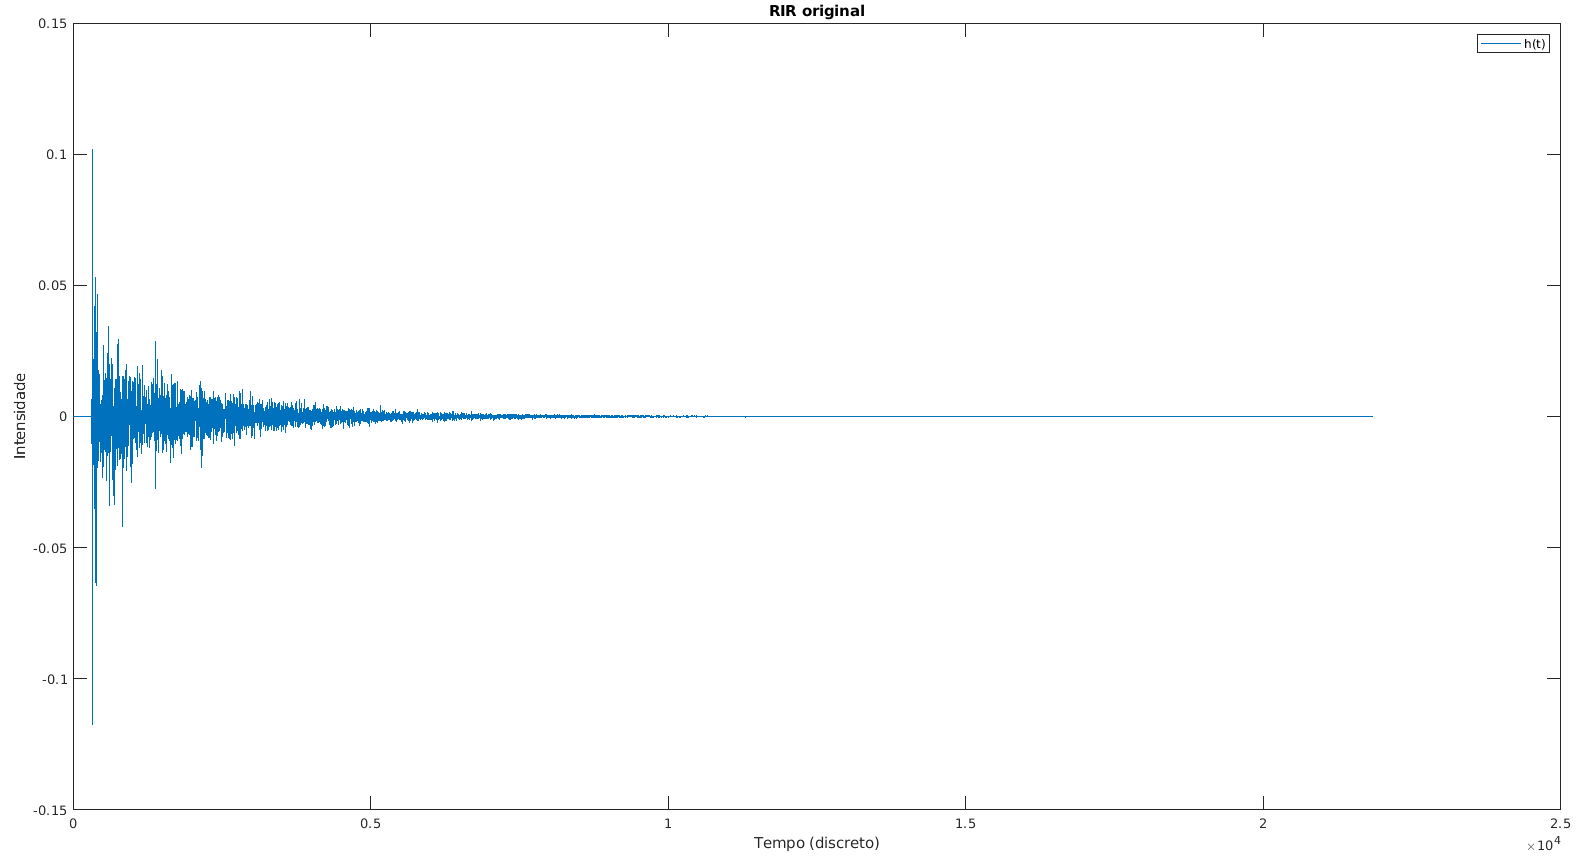
\includegraphics[scale=0.25]{rir-og-d1.png}
    \caption{RIR original do exemplo T2.}
    \label{fig:rir-og-t2}
\end{figure} 

\begin{figure} [H]
    \centering
    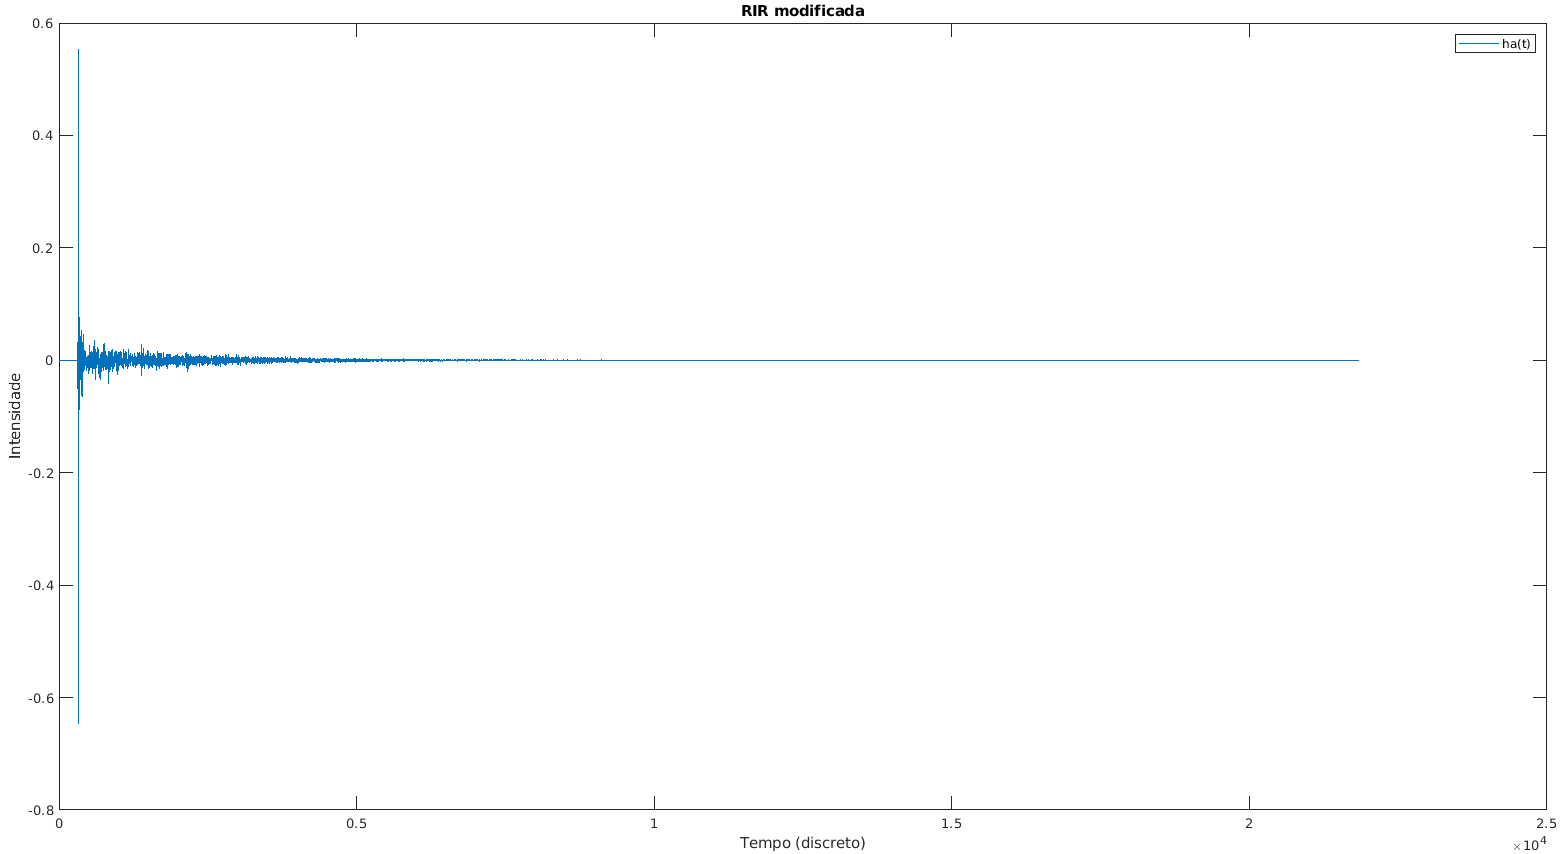
\includegraphics[scale=0.25]{rir-aug-d1.png}
    \caption{RIR simulada do exemplo T2.}
    \label{fig:rir-aug-t2}
\end{figure} 

De forma análoga aos resultados de DRR, foi feito um experimento empírico com o objetivo de medir o nível de “eco” do som, ou seja,
a sensação subjetiva do locutor estar falando em um espaço fechado mais amplo, gerando reverberação.
Foram geradas amostras de voz reverberadas (AVR) usando a RIROG e RIRSM e assim foram feitos dois testes subjetivos exibidos na tabela \ref{tbl:t60-exp}:
o primeiro, representado pela coluna “Comparação”, identifica qual das AVRs (a convoluída com RIROG ou a convoluída RIRSM) está com mais eco;
já o segundo, representado pela coluna “Ordem”, identifica a ordem de mais para menos eco entre as AVRs geradas com RIRSMs.

\begin{table} [H]
    \centering
    \caption{Análise subjetiva de eco.}
    \label{tbl:t60-exp}
    \begin{tabular}{c|c|c|c|c}

        \textbf{Exemplo} & 
        \textbf{$T60_{org}$ (s)} & 
        \textbf{$T60_{res}$ (s)} & 
        \textbf{Comparação} &
        \textbf{Ordem} \\
        \hline 

        T1 & 1,38 & 1,01 & original & 2 \\
        T2 & 1,01 & 1,89 & simulado & 1 \\
        T3 & 0,75 & 0,60 & original & 3 \\

    \end{tabular}
\end{table}

De acordo com a tabela \ref{tbl:t60-exp}, também foi possível identificar precisamente a diferença de variações do T60 para as RIRSMs,
mesmo ocorrendo o $\rho$ elevado para T1, indicando que a DA está ocorrendo, mesmo não atingindo o $T60_{alvo}$.


\subsection{\textit{Data Augmentation} de fala em campo distante}

Esta seção observa a eficácia da \textit{Data Augmentation} de AVCDs; para isso, foram gerados cinco exemplos de AVCDs, suas configurações
são exibidas na tabela \ref{tbl:da-noise}, onde além dos parâmetros explicados nas seções anteriores, é exibido o $SNR_{alvo}$ que representa
a razão SNR desejada entre a AVCD gerada e os SRP e SRF inseridos.

\begin{table} [H]
    \centering
    \caption{Exemplos de DA de AVCD gerados.}
    \label{tbl:da-noise}
    \begin{tabular}{c|c|c|c|c|c}

        \textbf{Exemplo} & 
        \textbf{Sala RIR} & 
        \textbf{Distância (m)} &
        \textbf{AVA} &
        \textbf{SRP} &
        \textbf{SRF} \\
        \hline 

        N1 & lecture & 7.1 & M2-T1 & RP-6 & RF-1 \\
        N2 & booth & 1 & H2-T1 & RP-12 & RF-4 \\
        N3 & office & 2 & H1-T1 & RP-4 & RF-4 \\
        N4 & meeting & 1.7 & M1-T2 & RP-11 & RF-2 \\
        N5 & stairway & 1 & H2-T1 & RP-7 & RF-4 \\

    \end{tabular}
    \bigbreak
    \bigbreak
    \begin{tabular}{c|c|c|c|c|c}

        \textbf{Exemplo} & 
        \textbf{$DRR_{org}$ (db)} & 
        \textbf{$DRR_{res}$ (db)} & 
        \textbf{$T60_{org}$ (s)} & 
        \textbf{$T60_{res}$ (s)} &
        \textbf{$SNR_{alvo}$} \\
        \hline 

        N1 & -4,5 & 17 & 1,38 & 0,56 & 5 \\
        N2 & 4,7 & 17 & 1,01 & 1,39 & 10 \\
        N3 & 0,5 & 14 & 0,75 & 0,60 & 14 \\
        N4 & 6,0 & 16 & 0,81 & 1,16 & 19 \\
        N5 & 5,0 & 18 & 2,70 & 3,68 & 3 \\

    \end{tabular}
\end{table}

Abaixo temos os gráficos relativos ao exemplo N2, contendo a amostra de voz original na figura \ref{fig:voice-og-n2}, a amostra de voz reverberada
com a RIRSM na figura \ref{fig:voice-aug-n2} e a amostra de voz em campo distante na figura \ref{fig:voice-ns-n2}.

\begin{figure} [H]
    \centering
    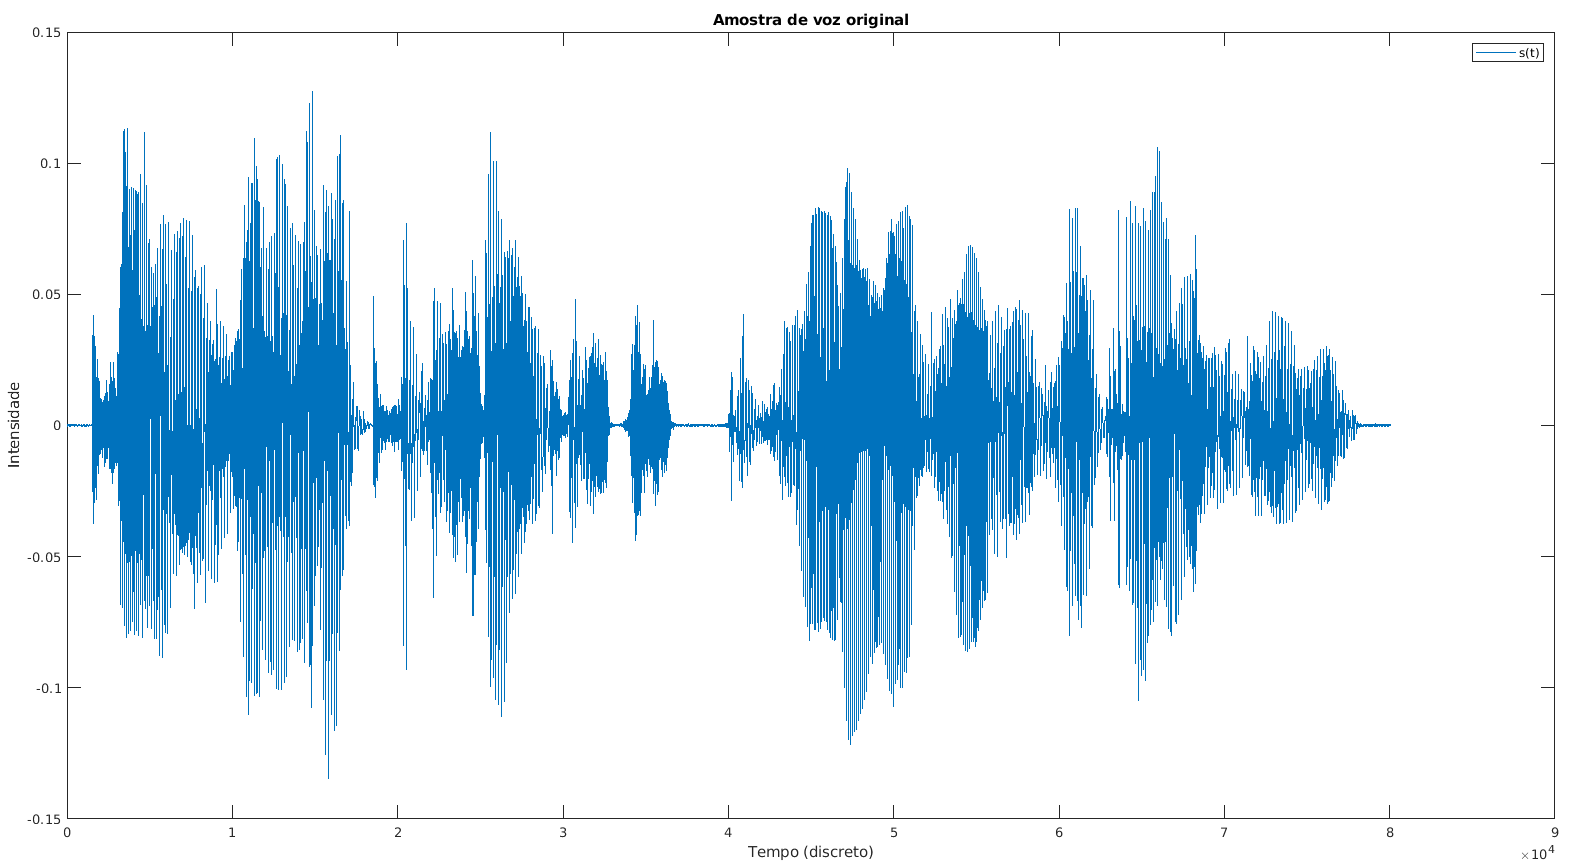
\includegraphics[scale=0.25]{voice-og-n2.png}
    \caption{Amostra de voz original no exemplo N2.}
    \label{fig:voice-og-n2}
\end{figure} 

\begin{figure} [H]
    \centering
    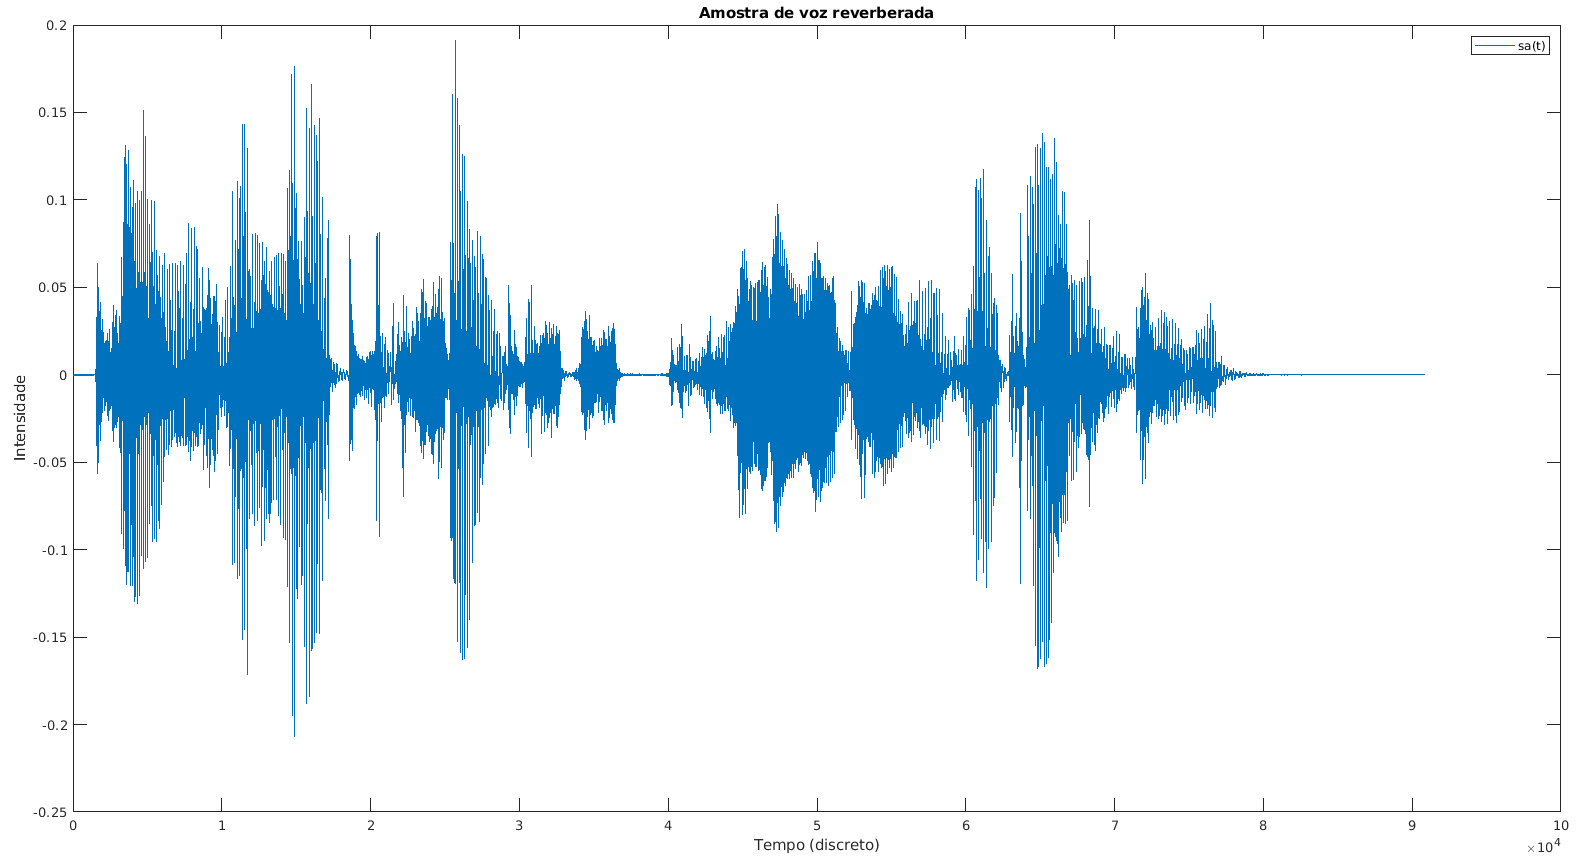
\includegraphics[scale=0.25]{voice-aug-n2.png}
    \caption{Amostra de voz reverberada com RIRSM no exemplo N2.}
    \label{fig:voice-aug-n2}
\end{figure} 

\begin{figure} [H]
    \centering
    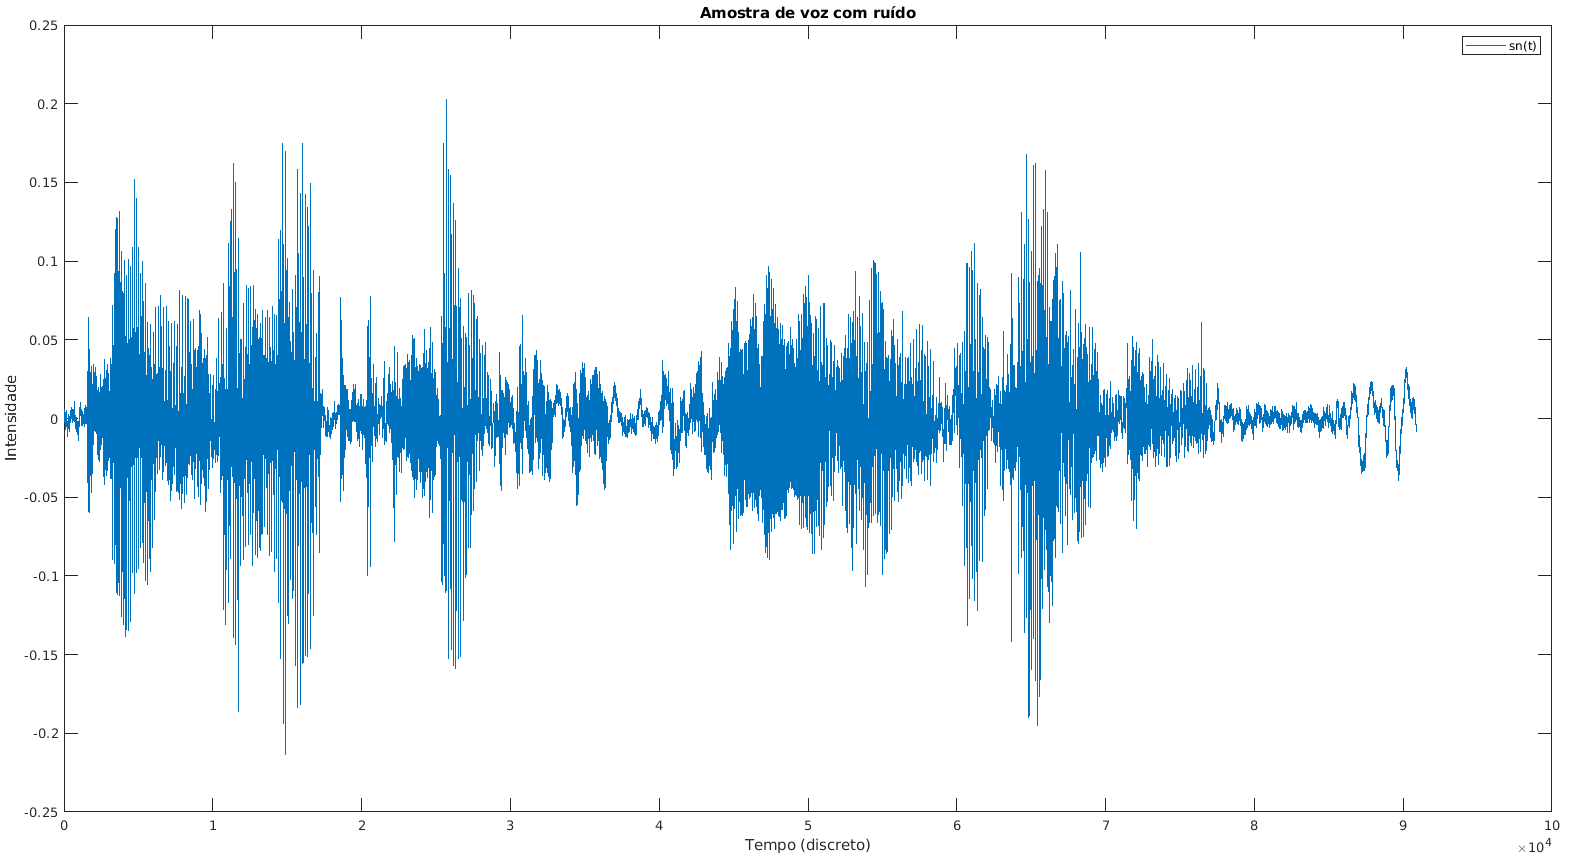
\includegraphics[scale=0.25]{voice-ns-n2.png}
    \caption{Amostra de voz em campo distante no exemplo N2.}
    \label{fig:voice-ns-n2}
\end{figure} 

Conforme o esperado, observa-se que a figura \ref{fig:voice-ns-n2} possui um ruído de chão claramente visível comparado à figura \ref{fig:voice-aug-n2}.
Nota-se também que na faixa de tempo entre 2000 e 4000 há picos sonoros que não são observados na amostra reverberada, estes picos representam o ruído pontual
introduzido no sinal.

De forma análoga, foi feito outro experimento empírico com o objetivo de medir o nível de ruído do som, ou seja, 
a sensação subjetiva de dificuldade de entender a fala do locutor devido aos outros sons misturados na amostra de voz.
Foram usados as cinco AVCDs apresentadas nesta seção e o teste subjetivo é exibido na tabela \ref{tbl:noise-exp}, onde
a coluna “Ordem”, identifica a ordem de mais para menos ruído entre as AVCDs geradas.

\begin{table} [H]
    \centering
    \caption{Análise subjetiva de nível de ruído.}
    \label{tbl:noise-exp}
    \begin{tabular}{c|c|c}

        \textbf{Exemplo} & 
        \textbf{$SNR_{alvo}$ (s)} & 
        \textbf{Ordem} \\
        \hline 

        N1 &  5 & 3 \\
        N2 & 10 & 4 \\
        N3 & 14 & 1 \\
        N4 & 19 & 5 \\
        N5 &  3 & 2 \\

    \end{tabular}
\end{table}

Observa-se que, em grande parte, os ruídos foram ordenados corretamente de nível decrescente de ruído, onde a única exceção foi o exemplo N3 votado como 
o mais ruidoso. De acordo com a pessoa que realizou os testes, o exemplo N3 possui um ruído pontual
de longa duração (neste caso representado pelo ruído “porta abrindo”), e isso atrapalhou no reconhecimento da fala do locutor.
